\documentclass[9pt]{article}
\usepackage{makeidx}
\usepackage{multirow}
\usepackage{multicol}
\usepackage[dvipsnames,svgnames,table]{xcolor}
\usepackage{graphicx}
\usepackage{epstopdf}
\usepackage{ulem}
\usepackage{hyperref}
\usepackage{amsmath}
\usepackage{amssymb}
\author{kalawa}
\title{}
\usepackage[paperwidth=595pt,paperheight=841pt,top=70pt,right=70pt,bottom=70pt,left=70pt]{geometry}

\makeatletter
	\newenvironment{indentation}[3]%
	{\par\setlength{\parindent}{#3}
	\setlength{\leftmargin}{#1}       \setlength{\rightmargin}{#2}%
	\advance\linewidth -\leftmargin       \advance\linewidth -\rightmargin%
	\advance\@totalleftmargin\leftmargin  \@setpar{{\@@par}}%
	\parshape 1\@totalleftmargin \linewidth\ignorespaces}{\par}%
\makeatother 

% new LaTeX commands


\begin{document}


{\raggedright
Chapitre
}

{\raggedright
Document
}

\begin{figure}[h]
\begin{center}
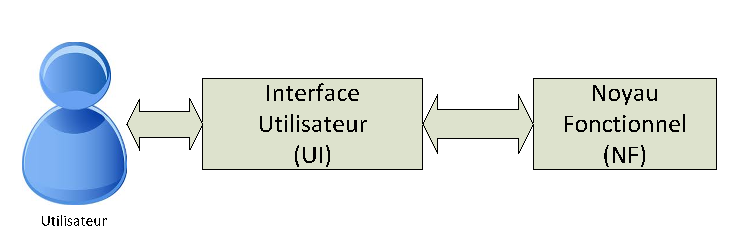
\includegraphics[width=406pt]{img-1.eps}
\caption{Application de consultation des contacts}
\end{center}
\end{figure}


\end{document}